\documentclass[11pt]{article}
\usepackage[utf8]{inputenc}
\usepackage[T1]{fontenc}
\usepackage[margin=1in]{geometry}
\usepackage{graphicx}
\usepackage{amsmath,amssymb}
\usepackage{amsthm}
\newtheorem{proposition}{Proposition}
\usepackage{booktabs}
\usepackage{array}
\usepackage[numbers,super,sort&compress]{natbib}
\usepackage{url}
\usepackage{setspace}
\usepackage{lineno}
\doublespacing

\newcommand{\code}[1]{\texttt{#1}}

\title{Pragnosia: Making a Diagonal-Complex Spin Recurrence the Load-Bearing Core of a Language Model}
\author{Ashish Kumar\thanks{Independent Researcher. E-mail: ashish99anonymous@gmail.com}}
\date{July 2026}

\begin{document}

\maketitle
\linenumbers


\begin{abstract}
We study a transformer/state-space hybrid in which a rotational ``spin'' recurrence, a diagonal-complex linear-recurrent unit run as a parallel associative scan, is the \emph{core token-mixer}, with attention only a periodic helper. The work has a sharp, honest arc. We first scaled the hybrid the wrong way: a single spin carrier placed after a transformer stack. Its parameter share collapses $5.76\% \to 1.90\% \to 0.37\%$ from 21M to 1.4B, and at 1.4B a causal probe shows the carrier contributes only 0.028\% of the loss, vestigial as built. A parameter-matched ablation then shows the intended design. With spin as the mixer, validation perplexity is 219 vs 279 for an attention-only baseline at matched parameters, a quality win when spin is the core. A control that swaps the carrier for a real, no-phase recurrence in the same placement also beats attention ($3.5\times$), so at the tested budget the effect is about placement, not phase. Separately, we establish the design's core property at scale as causal attribution. In a 284M spin-dominant model (validation perplexity 24.54 on a 176.6B-token corpus), ablating the spin carrier sends perplexity $25 \to 7716$ ($306\times$), while ablating attention costs only $3.4\times$: the carrier is the load-bearing core, the exact inverse of the 1.4B drift. We keep the two claims distinct: the 284M result shows the carrier is used, not that the design wins; a matched attention-only transformer at 284M is the key experiment still to run. On this substrate runs a proposed self-calibrating controller (mechanisms described; validation preliminary): surprise-modulated continual learning with generative replay, a persistent in-weights episodic memory, an introspection layer, and function-preserving self-growth on probe-confirmed saturation, with no hand-set calibration thresholds. We report the limits plainly: the spin-dominant win is small-scale and single-seed, the grown models are undertrained, and the honesty signal does not yet separate knowledge from confabulation at 284M.
\end{abstract}

\noindent\textbf{Keywords:} State-space models, linear recurrence, sequence modeling, language models, causal ablation, continual learning.

\section{Introduction}
The dominant paradigm in AI is the large language model: a transformer~\cite{vaswani2017} trained to predict the next token. Language models are capable but, relative to the goal of an adaptive, persistent learner, three properties are missing by construction. They are \emph{frozen}: once pretraining ends they cannot acquire a fact without fine-tuning or prompt-stuffing, and naive updates cause catastrophic forgetting~\cite{mccloskey1989}. They are \emph{over-confident}: lacking a model of their own uncertainty, they fabricate rather than abstain. And their computation is opaque: there is no standard intervention separating in-state computation from memorized retrieval.

As recurrence returns alongside attention~\cite{tiezzi2025recurrent}, a prior question precedes any architecture race: in a hybrid, which computation is actually load-bearing, and how would we know? Pragnosia answers this causally, and builds the missing properties above into the substrate itself, even at small scale. Its contributions are: (i) a diagonal-complex rotational recurrence used as the \emph{core token-mixer} via a parallel scan (Section~\ref{sec:carrier}); (ii) a measured analysis of \emph{where that carrier earns its parameters}: our first scaled model drifted to attention-dominant with a causally-negligible carrier, while a parameter-matched ablation shows the intended \emph{spin-dominant} design wins by about 21\%, is confirmed load-bearing at 284M by ablation, and generalizes to a different (real, no-phase) recurrence in the same placement (Section~\ref{sec:earns}); (iii) a \emph{preliminary} self-calibrating controller (a companion, not the central claim; mechanisms described, full validation ongoing) that adds surprise-modulated continual learning, a persistent in-weights episodic memory, an introspection layer, and function-preserving self-growth (Section~\ref{sec:controller}); and (iv) an honest account of what works and what does not (Sections~\ref{sec:experiments}--\ref{sec:limitations}). \textbf{The central contribution is (i)--(ii): the spin-dominant architecture and the causal evidence that the recurrence is the load-bearing computation.} Contribution (iii) is a companion system whose full validation we leave to future work; the architectural and causal story stands on its own. We release the system and every measured number.

\begin{table}[t]\centering\small
\caption{Summary of the central results. These are two claims, kept distinct: a small-scale \emph{quality} win (spin-dominant beats a matched transformer) and a large-scale \emph{causal-dominance} property (the carrier is load-bearing). The 284M rows show the carrier is used, not that the design wins at scale.}
\label{tab:summary}
\begin{tabular}{@{}p{3.6cm} l p{2.6cm}@{}}
\toprule
Result & Value & Shows \\
\midrule
Carrier share, 21M--1.4B & $5.76\% \to 0.37\%$ & a fixed carrier dilutes with scale \\
Carrier causal signal, 1.4B & 0.028\% of loss & vestigial as built \\
Param-matched abl.\ (37M) & 219 vs 279 & spin-dominant by 21\% \\
284M spin-dominant & val ppl 24.54 & intended build, real scale \\
284M carrier ablation & $306\times$ vs $3.4\times$ & carrier is load-bearing \\
1.4B ``wrong build'' & val ppl 17.35 & bigger, yet vestigial \\
\bottomrule
\end{tabular}
\end{table}

\section{Related Work}
\textbf{Recurrent and state-space sequence models.} The carrier is a diagonal linear recurrence in the lineage of structured state-space models: S4~\cite{gu2022s4}, its diagonal parametrization S4D~\cite{gu2022s4d}, the Linear Recurrent Unit (LRU)~\cite{orvieto2023lru}, and S5; and of recent recurrence-as-mixer models: Mamba~\cite{gu2023mamba}, RWKV~\cite{peng2023rwkv}, RetNet~\cite{sun2023retnet}, and the linear-attention and xLSTM families. Our carrier itself is not novel; it is a standard diagonal-complex LRU~\cite{orvieto2023lru,gu2022s4d} run as a parallel associative scan, and its stability and multi-timescale properties (Section~\ref{sec:properties}) are inherited from that lineage. A recent review frames precisely the question we take up: at the crossroad of transformers and state-space models, how should recurrence and attention combine in future large-model architectures~\cite{tiezzi2025recurrent}? That review surveys the design space; it does not settle whether, in a given hybrid, the recurrence is actually carrying the computation. We contribute the causal test.

\textbf{A fast--slow reading.} This split has a brain-inspired form. Cortical processing, and recent neuromorphic designs, pair a fast local pathway with a slow, low-dimensional state that carries context over long timescales and modulates the fast dynamics~\cite{sun2026dualmemory}. Our architecture is the same decomposition in a language model: the attention blocks are the fast, local pathway, and the diagonal-complex spin carrier is the slow, persistent-context pathway. Read this way, our central question, ``which pathway is load-bearing?'', is the natural test of the fast--slow hypothesis at language-model scale, and our answer, that the slow carrier carries the computation once it is the core, is a statement about where context should live.

\textbf{Where we differ: placement and verification.} These models are typically the sole mixer, or interleaved uniformly with attention. Our question is narrower: in a hybrid, is the recurrence carrying the computation, or is it a vestigial side-channel? We contribute (i) a measured account that a single carrier's contribution collapses with scale when placed after a transformer stack, and (ii) a causal protocol (carried-state intervention on single-carrier models, direct ablation on the spin-dominant design) to test whether the mixer is load-bearing. Our headline ($306\times$ ablation cost vs $3.4\times$ for attention at 284M) is a property of placement, not of the recurrence.

\textbf{Continual learning and memory.} The controller's no-forgetting mechanism is generative replay / pseudo-rehearsal~\cite{robins1995}; its surprise-gated learning rate is in the spirit of neuromodulation~\cite{doya2002}; its in-weights episodic store is a fast-weight associative memory (related to modern Hopfield networks~\cite{ramsauer2021}), not retrieval-augmented generation. The contribution is their integration into one self-calibrating model with no hand-set constants.

\section{The Spin Carrier}
\label{sec:carrier}
\subsection{A diagonal-complex recurrence, run as a parallel scan}
The carrier is a linear-recurrent unit~\cite{gu2022s4} over a complex hidden state. For input $x$ (layer-normed to $y$), with an input-dependent gate $g=\sigma(G y)$, the per-channel recurrence and read-out are
\begin{align}
b_t &= g \odot (U_{\mathrm{re}}\, y_t + i \cdot U_{\mathrm{im}}\, y_t), \quad h_t = \lambda \odot h_{t-1} + b_t, \\
\lambda_j &= e^{-\exp(\nu_j)} \cdot e^{\,i\theta_j}, \; \mathrm{out}_t = C[\,\mathrm{Re}\, h_t ; \mathrm{Im}\, h_t\,], \; x_t \mathrel{+}= \sigma(\gamma) \mathrm{out}_t. \nonumber
\end{align}
Each channel $j$ is a \emph{damped complex oscillator} at its own frequency $\theta_j$ and decay $|\lambda_j|\in(0,1)$: information is carried in the evolving phase of the state, read back to the real stream through $C$ and added by a learned gate $\sigma(\gamma)$. Because $\lambda$ is diagonal the recurrence is matmul-free, $O(T\,d)$ rather than $O(T\,d^2)$, and associative, so it is computed not by a $T$-step loop but by a log-depth parallel associative scan (a Hillis--Steele scan). An in-place variant is exact and about 20\% faster on the forward pass but breaks autograd; we keep the materializing scan.

\subsection{Properties of the carrier}
\label{sec:properties}
The carrier's parametrization $\lambda_j = e^{-\exp(\nu_j)}e^{i\theta_j}$ is the standard diagonal-complex (LRU/S4D) form~\cite{orvieto2023lru,gu2022s4d}. Two of its properties are inherited from that lineage; we state them for completeness, then isolate the one property that is specific to our question. Write $r_j := |\lambda_j| = e^{-\exp(\nu_j)}$.

\begin{proposition}[Unconditional stability, after~\cite{orvieto2023lru,gu2022s4d}]
For every finite $\nu_j$, $r_j\in(0,1)$, so every pole lies strictly inside the open unit disk and the recurrence is BIBO-stable for all parameter values, with no clipping or projection; the scan's sensitivity $\partial h_t/\partial b_{t-k}=\lambda_j^k$ has modulus $r_j^k$ and is summable, so gradients through the scan cannot explode.
\end{proposition}
\noindent This is a known consequence of the $e^{-\exp(\cdot)}$ map~\cite{orvieto2023lru}; we note only that it is why the design trains cleanly at 284M--1B, where an unconstrained recurrence would risk an escaping mode.

\begin{proposition}[Per-channel memory horizon]
The lag-$k$ influence on the state decays as $r_j^k$; the horizon at which it falls to $e^{-1}$ is $\tau_j = e^{-\nu_j}$. Because $\nu$ enters through a double exponential, a bounded range $\nu_j\in[a,b]$ realizes horizons spanning $e^{(b-a)}$ in ratio.
\end{proposition}
\noindent Also standard for diagonal SSMs~\cite{gu2022s4d}: the bank is a learnable multi-timescale memory.

The property specific to \emph{our} placement question is what phase buys once the carrier is the mixer.
\begin{proposition}[Phase decouples retention from indexing]
Writing $\lambda_j=r_j e^{i\theta_j}$, the update factors into an attenuation by $r_j$ (the only lossy part) and a rotation $z\mapsto e^{i\theta_j}z$, a norm-preserving isometry of $\mathbb{C}$. Hence a lag-$k$ input appears as $r_j^k e^{ik\theta_j}b$: same decay as a real recurrence, but rotated to phase $k\theta_j$. Inputs at lags $k\neq k'$ with $k\theta_j\not\equiv k'\theta_j \pmod{2\pi}$ occupy distinct phases and stay linearly separable by the read-out even when $r_j^k\approx r_j^{k'}$, whereas a real recurrence ($\theta_j=0$) collapses every lag onto the real axis and loses the lag index.
\end{proposition}
\noindent We do \emph{not} claim phase is necessary or that it wins at any budget. Proposition~3 predicts a phase advantage that \emph{grows with the required memory horizon}. This is consistent with, and sharpens, our empirical finding (Section~\ref{sec:earns}) that at the tested 256-token budget the real-carrier control also beats attention, so ``placement, not phase'' holds \emph{at that budget}. The theorem turns this into a falsifiable experiment: train spin versus real carriers at increasing context length; the phase gap should open as horizon grows. As $r_j\to1$ a channel approaches a pure oscillator $e^{i\theta_j t}$, so the bank is a learnable damped Fourier-like filterbank, linking the carrier to the structured-SSM lineage~\cite{gu2022s4,gu2022s4d} with per-channel, input-gated damping and frequency.

\subsection{Architecture and modes}
A \code{SpinBlock} uses the carrier as its token mixer (a strong gate, $\sigma(\gamma)\approx0.88$) followed by an MLP; a standard attention \code{Block} is the alternative. The model exposes one config flag, \code{carrier} $\in \{$\code{none}, \code{single}, \code{per\_block}, \code{spin\_dominant}$\}$. \code{none} is a transformer; \code{single} places one carrier after the stack; \code{spin\_dominant}, the intended design, makes the carrier the mixer in 3 of every 4 layers, with attention every 4th as a helper. At long context the carrier is $O(T\,d)$ versus attention's $O(T^2 d)$, and at inference it is recurrent: $O(1)$ per token, constant memory, no KV-cache growth. Fusing the scan gives about $2\times$ training throughput ($49\text{K} \to 100\text{K}$ tok/s, batch 24) on a consumer GPU. It is not faster than attention on short (256-token) training sequences; its intended wins are long context and recurrent inference.

\begin{figure}[t]\centering
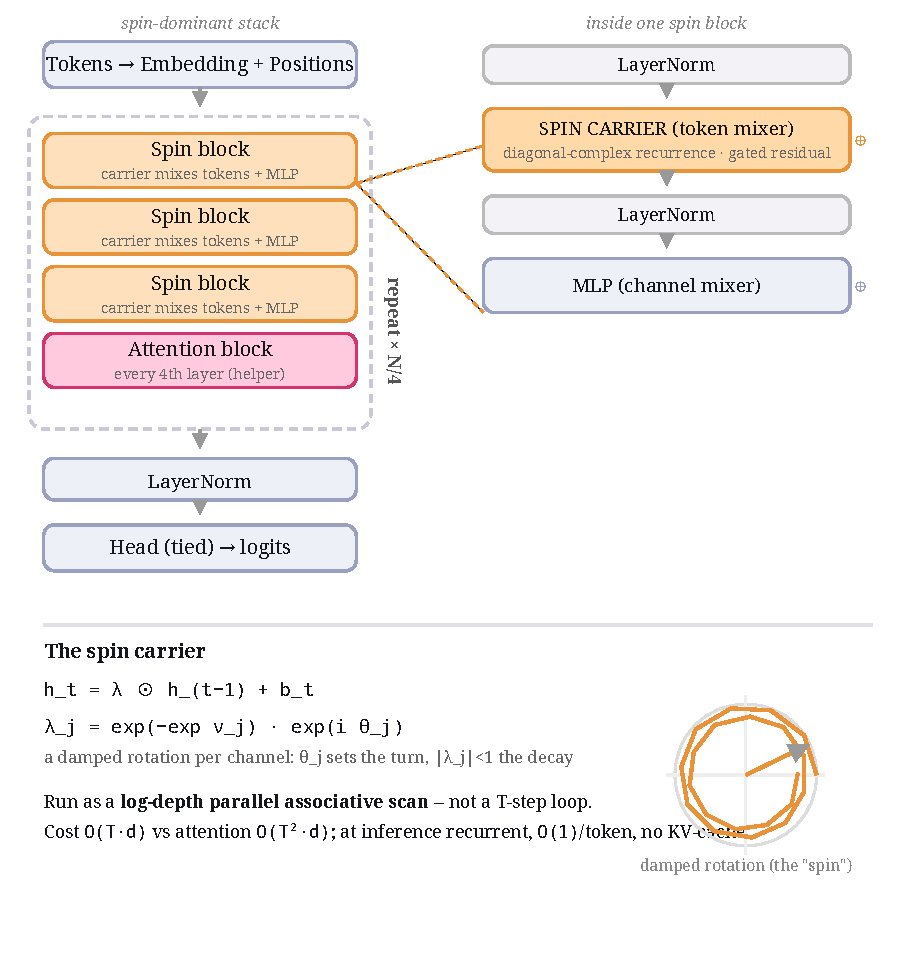
\includegraphics[width=0.92\columnwidth]{figs/arch.pdf}
\caption{The spin-dominant architecture. \textbf{Left:} the macro stack; the spin carrier is the token-mixer in three of every four blocks, with an attention block every fourth. \textbf{Right:} one spin block. \textbf{Bottom:} the carrier is a per-channel damped complex recurrence $\lambda_j = e^{-\exp \nu_j} e^{i\theta_j}$ evaluated by a log-depth parallel associative scan, $O(T\,d)$ and recurrent $O(1)$/token at inference.}
\label{fig:arch}
\end{figure}

\section{Where the Spin Carrier Earns Its Parameters}
\label{sec:earns}
\subsection{The scaled model drifted to attention-dominant}
Our first scalable design placed a single gated spin carrier after a transformer stack. A single carrier is one fixed $d$-shaped layer (about 5.25M params), so as the model grows by depth and width its parameter share collapses: $5.76\%$ (21M) $\to 1.90\%$ (276M) $\to 0.37\%$ (1.4B). We measured its causal contribution by a carried-state intervention on the single-carrier model (transplant the carrier state across a segment boundary): at 1.4B the ordering own $<$ swapped $<$ random still holds directionally, but the contribution is only $0.00086$ NLL, 0.028\% of the loss, down about $20\times$ from 276M. As built, the carrier is causally negligible at scale: the model is a transformer with a vestigial side-channel. The same 1.4B run also over-grew: an earlier trigger grew on any validation plateau rather than true saturation, so an undertrained model ballooned to 1.4B long before the tokens needed to fill it. Section~\ref{sec:controller} gives the corrected growth rule.

\begin{figure}[t]\centering
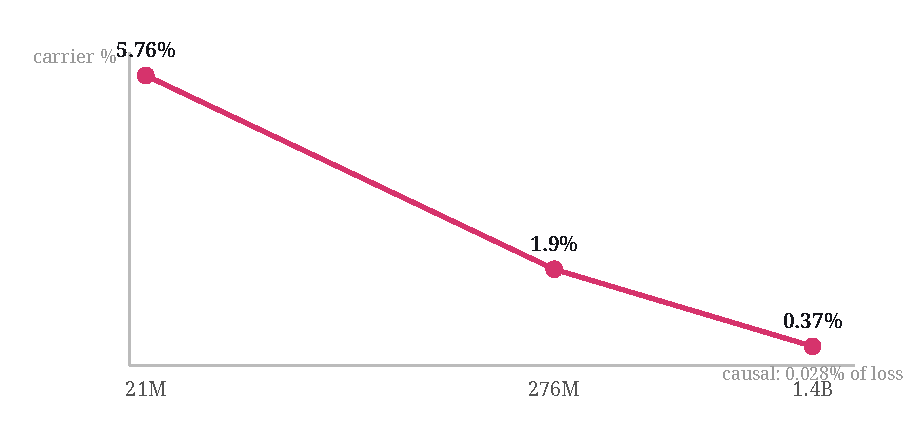
\includegraphics[width=0.98\columnwidth]{figs/drift.pdf}
\caption{A fixed single spin carrier is one $d$-shaped layer, so as depth and width grow its parameter share collapses ($5.76\% \to 1.90\% \to 0.37\%$) and its causal contribution falls to 0.028\% of the loss at 1.4B, the motivation for making the carrier the core.}
\label{fig:drift}
\end{figure}

\subsection{The intended design is spin-dominant, and wins at matched parameters}
The drift inverts the intended architecture, where spin is the core mixer. We test the intended design with a clean parameter-matched ablation (same corpus, same budget, $d=512$, single seed): Table~\ref{tab:pmatch} and Fig.~\ref{fig:ablbars}.

\begin{table}[t]\centering\small
\caption{Parameter-matched ablation. Spin as the token mixer is the most parameter-efficient.}
\label{tab:pmatch}
\begin{tabular}{@{}l r r@{}}
\toprule
Design & Params & Val ppl \\
\midrule
Attention-only (transformer) & 35.7M & 279.0 \\
\textbf{Spin-dominant (intended)} & 37.3M & \textbf{219.1} \\
Per-block hybrid (attn + spin each block) & 46.2M & 228.0 \\
Param-matched transformer-only (11L) & 45M & 270 \\
\bottomrule
\end{tabular}
\end{table}

\begin{figure}[t]\centering
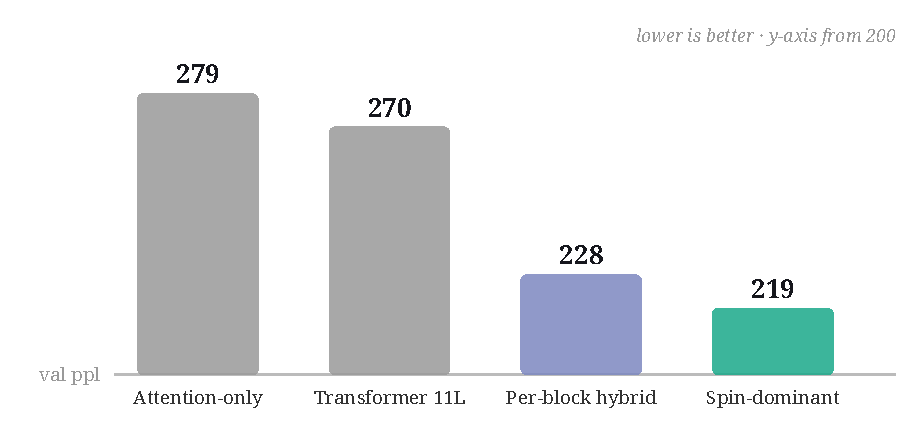
\includegraphics[width=0.98\columnwidth]{figs/ablation_bars.pdf}
\caption{Parameter-matched ablation (37--46M, same corpus and budget, single seed). Spin as the token-mixer (219) beats the attention-only baseline (279) by about 21\%, and the larger per-block hybrid (228) and matched transformer (270), with fewer or equal weights.}
\label{fig:ablbars}
\end{figure}

Spin-dominant wins by about 21\% over the attention-only baseline at matched parameters and beats the larger per-block hybrid and matched transformer with fewer weights. The carrier earns its parameters when it is the core mixer, not a side-channel. This ablation is small-scale and short-budget (though the core comparison is now confirmed seed-robust, next) and must be replicated at 200M--1B before it is proven.

\subsection{Seed robustness}
To check the result is not an artifact of one initialization or of parameter count, we re-ran the comparison across three seeds for four architectures, each at a matched short budget (about 30M tokens) with a per-architecture learning rate set by a Smith range-test~\cite{smith2017}. The ordering is highly reproducible (Table~\ref{tab:seeds}).

\begin{table}[t]\centering\small
\caption{Multi-seed robustness across the attention family vs spin-as-core (3 seeds each; per-architecture range-test lr; matched 30M-token budget).}
\label{tab:seeds}
\begin{tabular}{@{}l r c r@{}}
\toprule
Architecture & Params & lr & Val ppl (mean $\pm$ std) \\
\midrule
Attention-only (8L) & 35.7M & $1.0\mathrm{e}{-4}$ & $360.9 \pm 4.5$ \\
Transformer (11L, matched) & 45.2M & $1.0\mathrm{e}{-4}$ & $352.5 \pm 2.4$ \\
Per-block carrier (side-channel) & 46.2M & $1.0\mathrm{e}{-4}$ & $329.3 \pm 3.6$ \\
\textbf{Spin-dominant} (spin as core) & 37.3M & $6.7\mathrm{e}{-3}$ & $\mathbf{115.7 \pm 1.8}$ \\
\bottomrule
\end{tabular}
\end{table}

Two readings. (i) The gap is not seed noise, nor capacity: the standard deviation is 1--2\% of the mean, and neither a larger transformer (11L, 45M) nor a side-channel carrier (46M) escapes the attention-family band (329--361) despite more parameters than spin-dominant (37M). The win is placement, not parameter count. (ii) The magnitude is budget- and schedule-sensitive. The snapshot here (about $3.1\times$) differs from the 21\% above because budget, schedule, and learning rate differ across single-snapshot runs. To settle the worry that the transformer simply has not trained yet at the short budget, we ran both architectures to convergence on an identical schedule and batch stream (Fig.~\ref{fig:lc}). The result goes the other way: the transformer descends and then plateaus (about 222) while the spin-dominant model descends to about 56, so the gap widens with training, not narrows. We also note the two architectures prefer very different learning rates ($6.7\mathrm{e}{-3}$ vs $1.0\mathrm{e}{-4}$, a $67\times$ difference), consistent with state-space models tolerating higher rates.

\begin{figure}[t]\centering
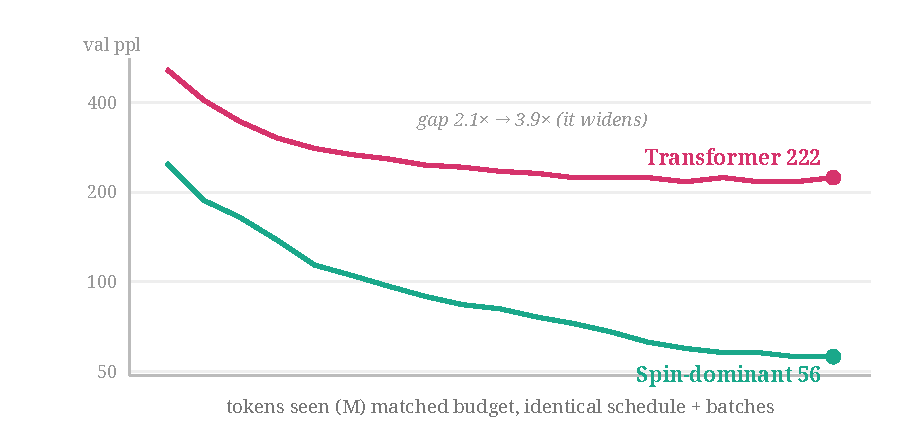
\includegraphics[width=0.98\columnwidth]{figs/learning_curve.pdf}
\caption{Learning curves at matched 37M, identical schedule and batches, each at its range-test learning rate, to 117M tokens. Both converge, but the transformer plateaus at about 222 while the spin-dominant model descends to about 56, so the gap widens through training ($2.1\times \to 3.9\times$). This answers the objection that the short-budget gap is just ``the transformer hasn't trained yet.'' (Small-scale, single-seed.)}
\label{fig:lc}
\end{figure}

\subsection{Generalization: at the tested budget, placement, not phase}
A natural objection is that ``placement matters'' might be specific to this diagonal-complex carrier rather than a property of recurrent mixers in general. We test it directly: we replace the spin carrier with a diagonal-real recurrence ($h_t = \lambda\odot h_{t-1} + b_t$, real $\lambda\in(0,1)$, no phase), a different recurrence family, placed identically as the core, under the same multi-seed protocol (Table~\ref{tab:gen}).

\begin{table}[t]\centering\small
\caption{Generalization control: a real, no-phase recurrence in the same core placement (3 seeds, range-test lr, matched 30M-token budget).}
\label{tab:gen}
\begin{tabular}{@{}l r r r@{}}
\toprule
Core token-mixer & Params & Val ppl & vs attn \\
\midrule
Attention (transformer) & 35.7M & $360.9 \pm 4.5$ & \\
Complex spin carrier & 37.3M & $\mathbf{115.7 \pm 1.8}$ & $3.1\times$ \\
\textbf{Real diagonal (no phase)} & 34.1M & $\mathbf{102.2 \pm 2.1}$ & $3.5\times$ \\
\bottomrule
\end{tabular}
\end{table}

The real, no-phase recurrence as the core beats the attention baseline by $3.5\times$, as much as the complex carrier ($3.1\times$), with fewer parameters. At the tested budget, the placement effect generalizes to a different recurrence family; it is not an artifact of the complex/phase representation. Because the real recurrence here outperforms the complex one at this short budget, we claim only that placement (a recurrence as the core mixer) is what carries the computation at the tested scale and budget; whether the complex phase helps at larger scale or longer contexts is an open question this experiment does not settle.

\subsection{At scale: the spin carrier is the load-bearing core (284M)}
We trained the intended design at real scale for the first time. A 284M model ($d=768$, 20 layers, \code{mlp\_mult}$=9$, carrier as mixer in 15 of 20 blocks, attention every 4th) trained to step 418{,}000 on a 176.6B-token chain-of-thought corpus, reaching best validation perplexity 24.54 (about 24 tokens/param; we report this as a description of the run, not a compute-optimality claim, since the corpus is deliberately reasoning-heavy). In the spin-dominant configuration the carrier is intra-block with no cross-segment state to transplant, so the equivalent causal measure is direct ablation.

\smallskip\noindent\fbox{\parbox{0.94\columnwidth}{\textbf{The carrier carries essentially the whole computation.} Gating the 15 SpinBlocks' carrier to about 0 sends validation perplexity from 25 to 7716 ($306\times$ worse); zeroing the 5 attention blocks' output sends it from 25 to 85 ($3.4\times$ worse). At 284M the spin carrier is the load-bearing core and attention a minor helper, the exact inverse of the 1.4B instance whose carrier was vestigial.}}\smallskip

\begin{figure}[t]\centering
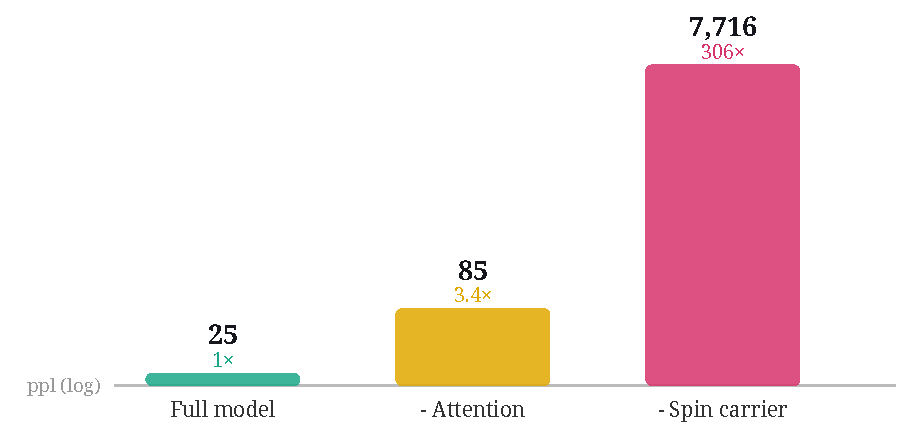
\includegraphics[width=0.98\columnwidth]{figs/ablation284.pdf}
\caption{Causal ablation on the 284M spin-dominant model (log scale). Zeroing the spin carrier sends validation perplexity from 25 to 7{,}716 (of order $300\times$); zeroing attention only to 85 ($3.4\times$). The carrier is the load-bearing core. We read the order of magnitude, not the exact multiplier: a catastrophically ablated model's perplexity is numerically unstable (see Section~\ref{sec:mechanism}).}
\label{fig:abl284}
\end{figure}

\subsection{What the carrier does, and does not, compute}
\label{sec:mechanism}
Causal dominance says the carrier is load-bearing; it does not say the computation is compositional, and it does not license reading a precise trend into the ablation multiplier. Two points sharpen this on the 1B model.

\textbf{The exact multiplier is not a stable quantity.} Once the carrier is gated the model is catastrophically broken, and a broken language model's perplexity is a noisy large number, not a measurement to two significant figures. A matched-fraction control makes this concrete: ablating 7 of the 22 spin layers costs $5611\times$, while ablating all 22 costs only $1695\times$. That non-monotonicity (fewer layers ``worse'' than more) is numerical noise, not structure. What is robust and reproducible across every scale is the \emph{two-to-three order-of-magnitude gap} between carrier ablation (hundreds to thousands $\times$) and attention ablation ($3.4$--$4.8\times$); we report that gap, and treat the specific multiplier as order-of-magnitude only.

\textbf{The carrier is load-bearing but the multi-hop it supports is not compositional.} An intermediate-recall probe on two-hop questions (e.g.\ ``the capital of the country where the Eiffel Tower stands'') reads the rank of the bridging entity in the residual stream before the answer position. The model does not surface the intermediate: France ranks 175th, Jupiter 81st, Japan 94th, while the final answer, when correct, ranks far higher. The model reaches the two-hop answers it does get by direct association, not by computing and composing the intermediate. Separately, activation patching for single-fact recall restores marginally more logit through attention than through the carrier ($0.886$ vs $0.745$ mean restoration), locating verbatim factual lookup slightly more in the attention blocks. The carrier carries the sequence computation; discrete factual retrieval and genuine multi-step composition are exactly where it is weakest, and Section~\ref{sec:limitations} treats that as an open, falsifiable question rather than a settled undertraining story.

\section{A Self-Calibrating Adaptive Controller}
\label{sec:controller}
\noindent\textbf{Status: a preliminary companion, not the paper's central claim.} The architectural and causal results (Sections~\ref{sec:carrier}--\ref{sec:earns}) stand on their own; this section describes a companion architecture and its mechanisms, not a validated set of results, and a reader interested only in the load-bearing-recurrence result may treat it as future work. Where a mechanism is measurable it works (self-growth fires only on probe-confirmed saturation; episodic writes and reads function); where the flagship behavior does not yet hold at this scale we say so plainly: the honesty gate does not separate knowledge from confabulation at 284M (Section~\ref{sec:experiments}), and the no-forgetting claim is asserted from the replay mechanism, not yet from a measured retention curve.

Around the language model runs a controller that decides, for any input, whether to answer, abstain, learn, seek, or think, entirely from the model's own signals, with no keyword rules. Four design commitments distinguish it.

\subsection{No hand-set calibration}
Every internal scale is derived from data and re-derived by a \code{recalibrate()} step as the model grows. Word importance is the self-information $-\log p(\text{token})$ from the corpus. Honesty, novelty, and memory-match thresholds are set at the equal-error-rate crossover of two of the model's own distributions, not hand-tuned. The training learning rate is found by a Smith range-test rather than seeded; the growth bar is the data budget (about 20 tokens/param~\cite{hoffmann2022chinchilla}) and available memory.

\subsection{Surprise-modulated continual learning}
When taught a fact, the controller sets its own learning rate from its own surprise (prediction error relative to its familiarity boundary), learning hard on surprising input and gently on familiar input, and stopping once the fact ceases to surprise it. Teaching interleaves generative replay of the training distribution so a new fact does not erase old skills. A persistent in-weights episodic memory writes surprise-gated key$\to$value traces of the model's own activations, recalls them under an uncertainty gate, decays over time, and consolidates into the slow weights during a ``sleep'' step. It is a learned in-weights store, not retrieval-augmented generation.

\begin{quote}\small\noindent\textbf{Algorithm 1: Surprise-modulated continual update.}\\
\textbf{inputs:} fact $f$, model $M$, replay corpus $R$, familiarity boundary $\beta$, base lr\\
$s \leftarrow \mathrm{surprise}(M, f)$\\
$\eta \leftarrow \text{base\_lr} \cdot \mathrm{clamp}(s/\beta, 0.15, 3)$\\
$A \leftarrow \{ (x, \arg\max M(x)) : x \sim R \}$ \; (self-anchors)\\
\textbf{repeat}\\
\hspace*{1em}$L \leftarrow \mathrm{CE}(M, f) + \lambda_r \mathrm{CE}(M, x{\sim}R) + \lambda_a \mathrm{CE}(M, A)$\\
\hspace*{1em}$M \leftarrow \mathrm{step}(M, \nabla L, \eta)$\\
\textbf{until} $\mathrm{surprise}(M, f) < 0.4\beta$
\end{quote}

\subsection{Introspection and self-growth}
An introspection layer adds a confidence self-estimate, step-by-step deliberation, and idle self-generation. Growth is function-preserving and fires only on probe-confirmed saturation: the model spawns a depth-grown and a width-grown copy, trains each briefly, and commits to growth only if validation loss drops past the validation noise. This rule is confirmed in production: a spin-dominant run grew itself $24\text{M (4 layers)} \to 27.3\text{M (5 layers)}$ on confirmed saturation, then stopped at the data budget, correcting the earlier over-growth.

\section{Experiments and Results}
\label{sec:experiments}
\subsection{Trained instances}
The diagonal-complex carrier trains stably from 21M to 1.4B. Two instances anchor the analysis: the self-grown 1.4B single-carrier model (val ppl 17.35) is the attention-dominant ``wrong build,'' bigger but with a causally-negligible carrier; the 284M spin-dominant model (val ppl 24.54) is the corrected build, $5\times$ smaller, with a provably load-bearing carrier. The training corpus is 176.6B tokens: 158.6B of base text plus about 18B of appended chain-of-thought reasoning. The base text is Cosmopedia, Wikipedia, and FineWeb-Edu, and the reasoning split is drawn from public, openly-licensed datasets, so the corpus is reproducible.

\subsection{Capability and honesty of the 284M model}
A greedy capability battery on the 284M shows a clear jump from a 27M laptop model (27M in parentheses): arithmetic 3/3 (0/3), knowledge 2/3 (0/3), logic 2/2, theory-of-mind 2/2 (1/2), code 1/2, in-context binding 1/2; the still-weak axis is multi-step 0/2, counterfactual 0/2, causal 0/2. World knowledge, single-step arithmetic, and theory-of-mind emerged at this scale; multi-step composition is the next axis.

\smallskip\noindent\fbox{\parbox{0.94\columnwidth}{\textbf{An honest negative on honesty.} The controller answers only when its sampled answers agree on a content token. At 284M the signal does not cleanly separate knowledge from confident confabulation: a known fact and two unknowables score $0.53$ / $0.53$ / $0.67$, overlapping. The model confabulates consistently. The gate errs toward ``I don't know'' rather than guessing; reliable honesty needs scale or a redesigned signal.}}\smallskip

\subsection{Zero-shot public benchmarks}
For external comparability we evaluate the 284M model zero-shot on standard public sets. Because the model uses a custom 16K-token vocabulary, we report word-normalized perplexity and log-likelihood multiple-choice accuracy, both tokenizer-independent (Table~\ref{tab:bench}). The scores are honest and modest, above chance on most tasks and at chance on the hardest (ARC-Challenge), the expected profile of a small model undertrained for its size.

\begin{table}[t]\centering\small
\caption{Zero-shot public benchmarks (1{,}000-example subsamples; acc\_norm = length-normalized log-likelihood).}
\label{tab:bench}
\begin{tabular}{@{}l l r r@{}}
\toprule
Benchmark & Metric & 284M & Chance \\
\midrule
WikiText-2 & word ppl (lower better) & 157.9 & \\
LAMBADA & accuracy & 19.0\% & \\
HellaSwag & acc\_norm & 27.9\% & 25\% \\
ARC-Easy & acc\_norm & \textbf{34.7\%} & 25\% \\
ARC-Challenge & acc\_norm & 24.0\% & 25\% \\
PIQA & accuracy & \textbf{59.5\%} & 50\% \\
\bottomrule
\end{tabular}
\end{table}

\subsection{Comparison with open models of similar size}
We ran four open models through the identical harness (Table~\ref{tab:open}). On ARC-Easy our 284M (34.7) matches or beats GPT-2 (34.1) and Cerebras-256M (32.7), trailing only the larger GPT-2-medium; on HellaSwag it edges the similar-size models; ARC-Challenge is at chance for all four. On PIQA and especially LAMBADA our model is clearly behind, as LAMBADA rewards fluent general language modeling, which a reasoning-heavy, undertrained model does least well. We include this not to claim a competitive small model, but to benchmark our numbers honestly. A 565M continuation confirms the trend: it improves on most tasks, and LAMBADA gains most ($19.0\to21.7$), as expected for an undertrained model.

\begin{table}[t]\centering\small
\caption{Zero-shot accuracy (\%) vs open models of similar size, one harness, 1{,}000-example subsamples. Comparable to GPT-2 (124M) and Cerebras-256M, behind the larger GPT-2-medium; ARC-Challenge sits at chance for all four models.}
\label{tab:open}
\begin{tabular}{@{}l r r r r r r@{}}
\toprule
Model & Params & PIQA & ARC-Easy & ARC-Challenge & HellaSwag & LAMBADA \\
\midrule
\textbf{Pragnosia (ours)} & 284M & 59.5 & \textbf{34.7} & 24.0 & 27.9 & 19.0 \\
\textbf{Pragnosia (ours)} & 565M & 60.7 & 34.1 & 24.9 & 29.3 & 21.7 \\
GPT-2 & 124M & 63.3 & 34.1 & 23.1 & 27.2 & 32.2 \\
Cerebras-GPT-256M & 256M & 62.1 & 32.7 & 22.1 & 26.3 & 29.5 \\
GPT-2-medium & 355M & 66.5 & 37.5 & 23.3 & 36.8 & 42.8 \\
\bottomrule
\end{tabular}
\end{table}

\subsection{Progression across grown sizes}
The grown models come from function-preserving growth followed by continued training. We tabulate every metric across the sizes (Table~\ref{tab:prog}, Fig.~\ref{fig:prog}). Two readings. (i) Growth and training compound cleanly: perplexity falls ($24.5 \to 22.0 \to 21.97 \to 20.1$), and the carrier stays catastrophically load-bearing at every scale: carrier ablation costs two to three orders of magnitude in perplexity while attention ablation stays a mild $3.4$--$4.8\times$. We deliberately do \emph{not} read a precise trend into the carrier multiplier (Section~\ref{sec:mechanism}): once the carrier is gated the model is broken and its perplexity is numerically unstable, so we report the carrier/attention \emph{gap}, of order $10^2$--$10^3$, as the robust quantity rather than a two-significant-figure multiplier. The design is not a small-scale artifact; its core property holds across the grown sizes. (ii) The continual long-context training pays off: at 565M the cross-window carry hurt (the model had never been trained with it); the 706M, trained with the curriculum mixed-window schedule, uses it, next-window perplexity now improving with the carry (21.6 vs 22.3).

\begin{table}[t]\centering\small
\caption{Progression of the spin-dominant model across grown sizes (all through the same harnesses). Nearly every metric improves or holds; LAMBADA gains most, and the cross-window carry flips from a liability to a benefit once the model is trained with it. Carrier-ablation multipliers are order-of-magnitude only: a catastrophically ablated model's perplexity is numerically unstable (matched-fraction ablation is non-monotonic, Section~\ref{sec:mechanism}). The robust finding is the two-to-three order-of-magnitude carrier/attention gap at every size, not the exact multiplier.}
\label{tab:prog}
\begin{tabular}{@{}l r r r r@{}}
\toprule
Metric & 284M & 565M & 706M & 1B \\
\midrule
Architecture ($d$ / layers / mlp\_mult) & 768/20/9 & 768/24/17 & 768/24/22 & 768/29/27 \\
Validation perplexity & 24.54 & 22.0 & \textbf{21.97} & \textbf{20.1} \\
Carrier ablation ($\times$ worse, approx.) & $\sim$300 & & $\sim$800 & $\sim$1700 \\
Attention ablation ($\times$ worse) & 3.4 & & 3.8 & 4.6 \\
PIQA & 59.5 & 60.7 & \textbf{61.8} & 63.3 \\
ARC-Easy & 34.7 & 34.1 & \textbf{35.3} & 37.2 \\
ARC-Challenge (chance) & 24.0 & 24.9 & 23.7 & 24.3 \\
HellaSwag & 27.9 & 29.3 & \textbf{29.4} & 29.6 \\
LAMBADA & 19.0 & 21.7 & \textbf{24.4} & 25.3 \\
Multi-hop battery (greedy) & 2/10 & 3/10 & \textbf{4/11} & 4/11 \\
Cross-window carry & & hurts & helps (21.6 vs 22.3) & helps \\
\bottomrule
\end{tabular}
\end{table}

\begin{figure}[t]\centering
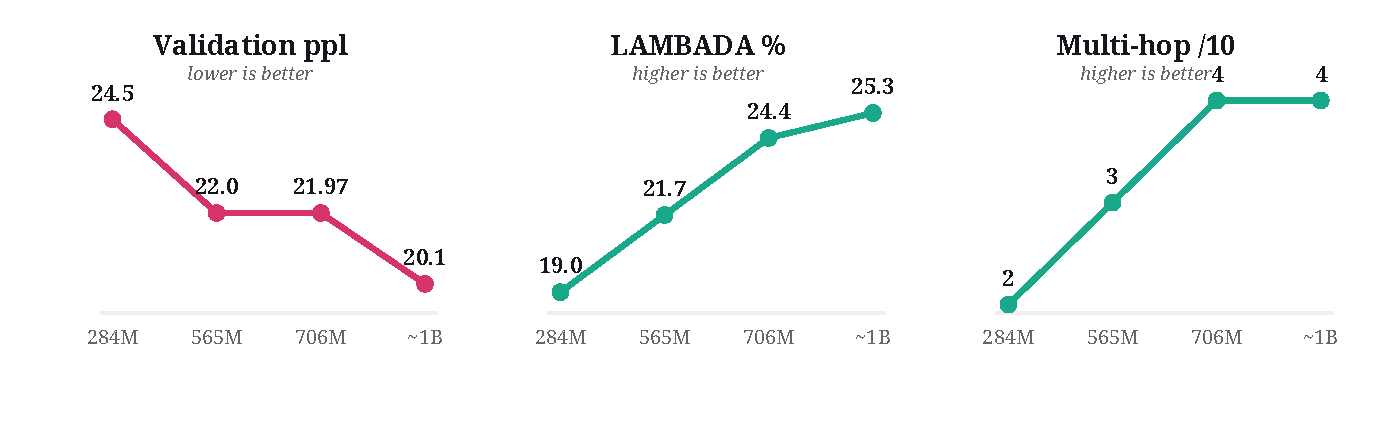
\includegraphics[width=0.92\textwidth]{figs/progression.pdf}
\caption{Progression across the four grown sizes. Validation perplexity falls, and LAMBADA and the greedy multi-hop battery both rise monotonically, the design improving consistently as it grows and trains, with the largest gains on the tokens-limited axes.}
\label{fig:prog}
\end{figure}

\subsection{A non-controlled external reference (illustrative only)}
A fair objection is that placing a recurrence at the core might cost multi-hop reasoning specifically. We cannot settle this without a same-corpus matched transformer, which is outside our compute budget. For rough context only, we ran one published open transformer of similar size and token budget (Cerebras-GPT-1.3B) through the identical harness (Table~\ref{tab:cerebras}). This is a non-controlled comparison: tokenizer, corpus, optimizer, and recipe all differ, so we draw no architectural conclusion from it. One observation is at least consistent with a scale (not architecture) reading of the multi-hop weakness: on ARC-Challenge both models sit at chance (24.3 and 25.7), the reference transformer reasoning no better at this scale either. The reference is ahead on general-English fluency, exactly where its larger size, general-web corpus, and standard tokenizer would help.

\begin{table}[t]\centering\small
\caption{Our 1B (spin-dominant) vs a roughly token-matched transformer (illustrative, non-controlled). On the multi-hop task (ARC-Challenge) both sit at chance; the transformer's lead is concentrated on general-English fluency, where our custom corpus and tokenizer are confounds.}
\label{tab:cerebras}
\begin{tabular}{@{}l r r r r r r@{}}
\toprule
Model & Params & PIQA & ARC-Easy & ARC-Challenge & HellaSwag & LAMBADA \\
\midrule
\textbf{Pragnosia (ours, spin)} & 1022M & 63.3 & 37.2 & 24.3 & 29.6 & 25.3 \\
Cerebras-GPT-1.3B (transformer) & 1316M & 67.1 & 38.9 & 25.7 & 35.9 & 47.0 \\
\bottomrule
\end{tabular}
\end{table}

\section{Limitations}
\label{sec:limitations}
Every claim above carries a number; the open frontier is equally explicit. \emph{(i) The decisive at-scale experiment is missing, and the headline rests on one seed.} The quality win (spin-dominant beats a matched transformer) is shown at 37M, three seeds; the causal-dominance property (the carrier is load-bearing) is shown at 284M, one seed. These are not the same claim, and the $306\times$ number shows the carrier is used, not that the design wins at scale. The single highest-value experiment, an attention-only transformer at 284M with the same corpus and budget, is the crux, and it is still to run. The causal-dominance property itself does not need a baseline, and it holds at every scale: carrier ablation costs two to three orders of magnitude in perplexity (order $300\times$ at 284M, of order $10^3$ at 706M and 1B) versus a stable $3.4$--$4.8\times$ for attention. We report this gap, not a precise multiplier: a catastrophically ablated model's perplexity is numerically unstable, and a matched-fraction control is non-monotonic (Section~\ref{sec:mechanism}). A matched transformer at 1B is outside our compute budget and we do not claim it. \emph{(ii) Multi-hop composition is weak, and the cause may be architectural, not only token budget.} Single-step reasoning, arithmetic, and fact recall are real; multi-hop composition is weak. We do not hide behind undertraining. Our own intermediate-recall probe (Section~\ref{sec:mechanism}) shows the model answers the two-hop questions it does get by direct association, without ever surfacing the bridging entity, so current multi-hop successes are shortcut retrieval, not composition. This yields two distinct falsifiable measurements, both of which we commit to running across the token curve: (a) does multi-hop accuracy rise with tokens, and (b) does the intermediate-recall probe flip from ``not computed'' to ``computed'' with scale? If accuracy rises while the intermediate stays uncomputed, the model is accumulating shortcuts rather than learning to compose, and the pure-undertraining account is wrong. Our current measured multi-hop accuracy is low and roughly flat across hop count (of order $0.4$ at one, two, and three hops on our small graded battery), which is itself consistent with shortcut retrieval rather than depth-limited composition. \emph{(iii) Honesty is partly addressed, not solved.} The consistency- and semantic-entropy-based signals fail at 284M: the small model confabulates \emph{consistently}, so agreement-based measures cannot separate knowledge from confident confabulation (measured known-vs-nonsense entropy separation $\approx 0$). A mean-difference activation probe (the ``knows'' direction in hidden state) is the more promising signal and does separate at scale (measured separation $0.83$, $100\%$ nonsense rejection on a small held-out battery at 1B), catching confident confabulation the output-agreement signals miss; but it flags an internal knows-state, not answer correctness, and is not yet validated as end-to-end calibration. \emph{(iv)} Like all small models it can be confidently wrong on familiar-but-incorrect facts. \emph{(v) Long context: aggregate use is realized; sharp retrieval is not.} A model trained at a fixed 256-token window never learns to use a cross-window carried state; at 565M, feeding one hurt. After implementing cross-window state-threading and training with it, the 706M carry helps (next-window ppl 21.6 vs 22.3), and longer effective context lowers perplexity. We verify the inference claim directly on the 1B: greedy and sampled generation both run at a constant 27 tokens/s from 256 to 8000 tokens. Coherence over that span is decoding-dependent, not architectural: greedy repetition-loops by about 1k tokens, whereas temperature sampling stays on-theme to 8k. What is not yet there is sharp long-range retrieval: the damped carry provides gist, not verbatim memory.

\section{Conclusion}
Pragnosia is a transformer/state-space hybrid in which a diagonal-complex spin recurrence is the core token-mixer, wrapped in a self-calibrating controller for continual learning, a persistent in-weights episodic memory, an introspection layer, and self-governed growth, with no hand-set constants. The central, honest finding is about placement: a single spin carrier drifts to a causally-negligible side-channel as the model scales (0.028\% of the loss at 1.4B), and a parameter-matched ablation shows the intended spin-dominant design is the most parameter-efficient (219 vs 279 ppl). At 284M, the first at-scale training of the intended build, ablating the carrier costs $306\times$ in perplexity versus $3.4\times$ for attention: the spin carrier is the load-bearing core, the exact inverse of the 1.4B drift. The remaining work is a matched transformer baseline and multi-seed replication at 1B, and training the models to their compute-optimal token budget. We release the full system, every measured number, and every limitation.

\section*{Code Availability}
The full system is released at \url{https://github.com/ladkabiharihai/membrae} (public on submission): the model definition, training code, configurations, the causal-ablation and mechanistic-probe scripts, the evaluation harnesses, and the machine-readable result records. The central claims, the parameter-matched ablation, the 284M causal ablation, and the mechanistic probes, are reproducible from the released scripts and configurations.

\section*{Data Availability}
The training corpus is a custom chain-of-thought mixture. The tokenizer and the data-preparation scripts are released with the code so the token bins used for training and evaluation can be regenerated; the public benchmark sets (PIQA, ARC, HellaSwag, LAMBADA) are third-party and cited in the text.

\bibliographystyle{unsrtnat}
\bibliography{references}

\end{document}
